\begin{center}
	
	\begin{tabular}{rp{16cm}lp{20cm}}%{rl}
		
		% after \\: \hline or \cline{col1-col2} \cline{col3-col4} ...
		
		论文地址:& \href{https://arxiv.org/pdf/1611.00144.pdf}{https://arxiv.org/pdf/1611.00144.pdf} \\
		来源:& ICDM, 2016 \\
		作者:& Yanru Qu, Han Cai, et al. \\
		
		%源码:& \href{xxx}{xxx} \\
		
		%  slides:& \href{http://yunshengb.com/wp-content/uploads/2017/03/nips_2018_r2l_workshop_talk.pdf}{{\footnotesize Convolutional Set Matching for Graph Similarity}}\\
		
		关键词:& \textbf{CTR, Deep Learning} \\
		
		写于:& \date{2021-09-06}
		
	\end{tabular}
	
\end{center}

该论文\cite{qu2016product-based}提出了一种新的层 --- Product-based Neural Networks,用于捕捉输入特征中不同域之间的交互模式。

\paragraph{问题定义}
解决CTR问题。已有的一些研究\cite{menon2011response, anhphuong2015factorization}表明Product操作有助于探索(explore)不同特征域之间关系。

\paragraph{PNN}
PNN整体结构如Fig.\ref{fig:pnn}所示。与其他的深度模型类似,每个输入的样本由多个field组成。经过Embedding Layer再输入到论文所提出的Product Layer。理一下模型的计算过程:
\begin{itemize}
	\item 原始输入$\boldsymbol{x}$被表示成$N$个filed,每个filed在$\boldsymbol{x}$中是$\boldsymbol{x}[start_i: end_i]$
	\item $\boldsymbol{x}$输入到Embedding Layer,进行field-wise,$field_i$的embedding为:$\boldsymbol{f_i} =\boldsymbol{W_0^i}\boldsymbol{x}[start_i: end_i]$
	\item Embedding Layer的输出进入Product Layer,这一层主要输出两个向量$\boldsymbol{l}_z, \boldsymbol{l}_p$,分别是\textbf{线性操作部分和乘积操作部分}。其中$\boldsymbol{z} = \{\boldsymbol{f_1}, ..., \boldsymbol{f_N}\},\: \boldsymbol{p} = \{p_{ij}\} = g(\boldsymbol{f_i}, \boldsymbol{f_j})$,其中$g$就是论文中提出的\textbf{Product}操作,$g$可以是内积也可以是外积。$\boldsymbol{l}_z = \boldsymbol{W}_z \boldsymbol{z}^T,\: \boldsymbol{l}_p = \boldsymbol{W}_p \boldsymbol{p}^p$,其中$\boldsymbol{W}_z \in \mathbb{R}^{D_1 \times N \times M},\: \boldsymbol{W}_p \in \mathbb{R}^{D_1 \times N \times N}$分别是Product Layer的权重,$D_1$是Hidden Layer1的神经元个数
	\item Product Layer的输出加上偏置$\boldsymbol{b_1}$一起输入Hidden Layer1,最终Hidden Layer1的输出:$\boldsymbol{l_1} = relu(\boldsymbol{l}_z + \boldsymbol{l}_p + \boldsymbol{b_1})$
	\item 接下来就是常规操作了,经过全连接层得到最终的输出,经过$sigmoid$得到预测值,作为CTR估计值
\end{itemize}


\begin{figure}[h]
	\centering
 	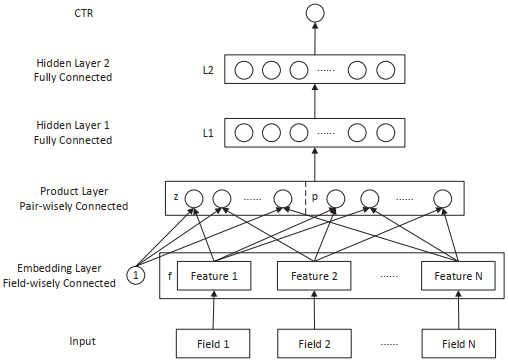
\includegraphics[width=.6\textwidth]{pics/pnn.png}
	\caption{PNN Architecture}
	\label{fig:pnn}
\end{figure}


\paragraph{关于Product操作}
$g$既可以是内积也可以是外积。当$g$是外积时,$g(\boldsymbol{f_i}, \boldsymbol{f_j})$就成了一个矩阵,为了降低时间复杂度和空间复杂度,论文中使用了叠加(Superposition)操作:
$$
\boldsymbol{p}=\sum_{i=1}^{N} \sum_{j=1}^{N} \boldsymbol{f}_{i} \boldsymbol{f}_{j}^{T}=\boldsymbol{f}_{\Sigma}\left(\boldsymbol{f}_{\Sigma}\right)^{T}, \quad \boldsymbol{f}_{\Sigma}=\sum_{i=1}^{N} \boldsymbol{f}_{i}
$$
实际上就是把所有field的embedding先求和再计算外积,最终依然得到$\mathbb{R}^{N \times N}$的矩阵。


\paragraph{总结}

\begin{itemize}
	\item $\boldsymbol{l}_z, \boldsymbol{l}_p$分别作为对特征的线性部分和特征交叉部分(有点Wide\&Deep的味道了)
	\item 外积操作进行了Superposition,对不同特征的对应维度求和,类似于对所有field的特征进行池化,这要求\textbf{不同特征的对应维度有相似的含义},\tbc{red}{但是不同field的embedding是通过不同的权重得到的 --- 位于不同的向量空间中,不同特征的同一维不具有可比性}
	
\end{itemize}

